\documentclass[14pt]{extbook}
\usepackage{multicol, enumerate, enumitem, hyperref, color, soul, setspace, parskip, fancyhdr} %General Packages
\usepackage{amssymb, amsthm, amsmath, bbm, latexsym, units, mathtools} %Math Packages
\everymath{\displaystyle} %All math in Display Style
% Packages with additional options
\usepackage[headsep=0.5cm,headheight=12pt, left=1 in,right= 1 in,top= 1 in,bottom= 1 in]{geometry}
\usepackage[usenames,dvipsnames]{xcolor}
\usepackage{dashrule}  % Package to use the command below to create lines between items
\newcommand{\litem}[1]{\item#1\hspace*{-1cm}\rule{\textwidth}{0.4pt}}
\pagestyle{fancy}
\lhead{Makeup Progress Quiz 1}
\chead{}
\rhead{Version B}
\lfoot{6018-3080}
\cfoot{}
\rfoot{Spring 2021}
\begin{document}

\begin{enumerate}
\litem{
Write the equation of the line in the graph below in Standard form $Ax+By=C$. Then, choose the intervals that contain $A, B, \text{ and } C$.
\begin{center}
    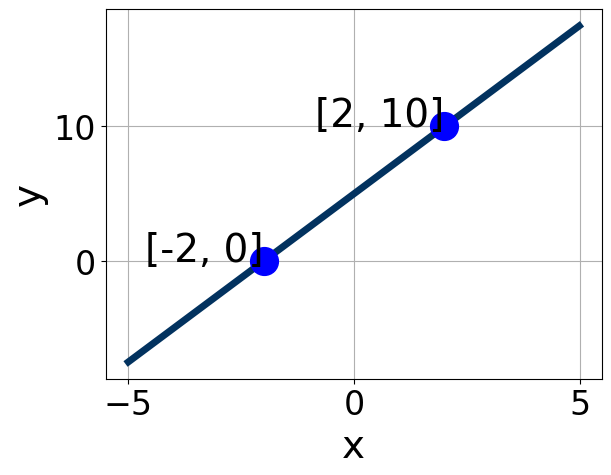
\includegraphics[width=0.5\textwidth]{../Figures/linearGraphToStandardCopyB.png}
\end{center}
\begin{enumerate}[label=\Alph*.]
\item \( A \in [3.1, 5.2], \hspace{3mm} B \in [-2.31, -1.18], \text{ and } \hspace{3mm} C \in [-10, -7] \)
\item \( A \in [-3.7, -2.4], \hspace{3mm} B \in [-1.2, -0.85], \text{ and } \hspace{3mm} C \in [-6, -2] \)
\item \( A \in [3.1, 5.2], \hspace{3mm} B \in [1.6, 2.12], \text{ and } \hspace{3mm} C \in [6, 11] \)
\item \( A \in [-6.7, -3.4], \hspace{3mm} B \in [1.6, 2.12], \text{ and } \hspace{3mm} C \in [6, 11] \)
\item \( A \in [-3.7, -2.4], \hspace{3mm} B \in [0.58, 1.57], \text{ and } \hspace{3mm} C \in [3, 6] \)

\end{enumerate} }
\litem{
Solve the linear equation below. Then, choose the interval that contains the solution.\[ \frac{-3x -3}{8} - \frac{6x -8}{3} = \frac{-3x -8}{7} \]\begin{enumerate}[label=\Alph*.]
\item \( x \in [0.88, 2.07] \)
\item \( x \in [6.57, 7.73] \)
\item \( x \in [-1.51, -0.61] \)
\item \( x \in [-0.43, 1.56] \)
\item \( \text{There are no real solutions.} \)

\end{enumerate} }
\litem{
Solve the equation below. Then, choose the interval that contains the solution.\[ -5(-7x + 4) = -17(3x + 11) \]\begin{enumerate}[label=\Alph*.]
\item \( x \in [-2.95, -2.23] \)
\item \( x \in [-2.19, -1.35] \)
\item \( x \in [-13.69, -12.92] \)
\item \( x \in [1.5, 2.69] \)
\item \( \text{There are no real solutions.} \)

\end{enumerate} }
\litem{
Find the equation of the line described below. Write the linear equation as $ y=mx+b $ and choose the intervals that contain $m$ and $b$.\[ \text{Perpendicular to } 9 x + 5 y = 15 \text{ and passing through the point } (-5, -9). \]\begin{enumerate}[label=\Alph*.]
\item \( m \in [0.25, 1.11] \hspace*{3mm} b \in [4.22, 9.22] \)
\item \( m \in [0.25, 1.11] \hspace*{3mm} b \in [-8.22, -5.22] \)
\item \( m \in [-1.22, -0.01] \hspace*{3mm} b \in [-13.78, -7.78] \)
\item \( m \in [1.37, 2.98] \hspace*{3mm} b \in [-8.22, -5.22] \)
\item \( m \in [0.25, 1.11] \hspace*{3mm} b \in [-4, 1] \)

\end{enumerate} }
\litem{
Write the equation of the line in the graph below in Standard form $Ax+By=C$. Then, choose the intervals that contain $A, B, \text{ and } C$.
\begin{center}
    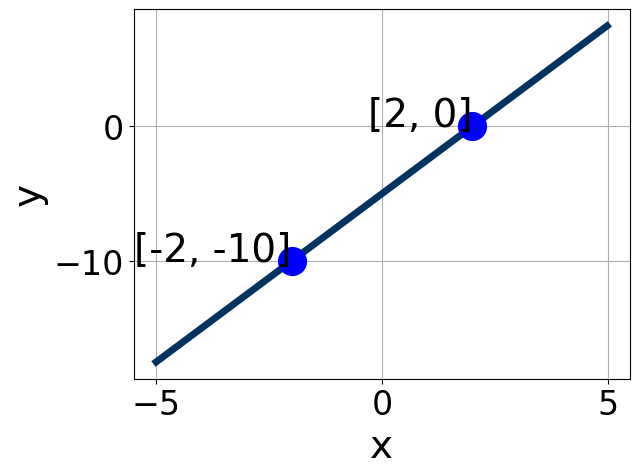
\includegraphics[width=0.5\textwidth]{../Figures/linearGraphToStandardB.png}
\end{center}
\begin{enumerate}[label=\Alph*.]
\item \( A \in [-4, 0.2], \hspace{3mm} B \in [-1.01, -0.42], \text{ and } \hspace{3mm} C \in [3, 7.6] \)
\item \( A \in [-4, 0.2], \hspace{3mm} B \in [-0.04, 1.63], \text{ and } \hspace{3mm} C \in [-6.1, -3.8] \)
\item \( A \in [-6.2, -4.5], \hspace{3mm} B \in [1.89, 2.65], \text{ and } \hspace{3mm} C \in [-10.4, -7] \)
\item \( A \in [4.2, 6.9], \hspace{3mm} B \in [1.89, 2.65], \text{ and } \hspace{3mm} C \in [-10.4, -7] \)
\item \( A \in [4.2, 6.9], \hspace{3mm} B \in [-2.84, -1.35], \text{ and } \hspace{3mm} C \in [9, 11.6] \)

\end{enumerate} }
\litem{
First, find the equation of the line containing the two points below. Then, write the equation as $ y=mx+b $ and choose the intervals that contain $m$ and $b$.\[ (9, -3) \text{ and } (3, 5) \]\begin{enumerate}[label=\Alph*.]
\item \( m \in [-13.33, 0.67] \hspace*{3mm} b \in [-10.31, -7.79] \)
\item \( m \in [-13.33, 0.67] \hspace*{3mm} b \in [-12.58, -10.87] \)
\item \( m \in [1.33, 4.33] \hspace*{3mm} b \in [0.44, 1.27] \)
\item \( m \in [-13.33, 0.67] \hspace*{3mm} b \in [8.18, 9.67] \)
\item \( m \in [-13.33, 0.67] \hspace*{3mm} b \in [1.49, 2.97] \)

\end{enumerate} }
\litem{
Solve the linear equation below. Then, choose the interval that contains the solution.\[ \frac{-7x -4}{7} - \frac{4x -8}{5} = \frac{-6x -7}{8} \]\begin{enumerate}[label=\Alph*.]
\item \( x \in [-0.2, 1.5] \)
\item \( x \in [1.6, 3.2] \)
\item \( x \in [-1.8, -0.9] \)
\item \( x \in [8.7, 13.3] \)
\item \( \text{There are no real solutions.} \)

\end{enumerate} }
\litem{
Solve the equation below. Then, choose the interval that contains the solution.\[ -12(6x + 18) = -2(-3x + 9) \]\begin{enumerate}[label=\Alph*.]
\item \( x \in [-3.57, -3.31] \)
\item \( x \in [-3.04, -2.93] \)
\item \( x \in [-2.94, -2.47] \)
\item \( x \in [2.86, 3.53] \)
\item \( \text{There are no real solutions.} \)

\end{enumerate} }
\litem{
Find the equation of the line described below. Write the linear equation as $ y=mx+b $ and choose the intervals that contain $m$ and $b$.\[ \text{Parallel to } 5 x + 6 y = 6 \text{ and passing through the point } (4, -10). \]\begin{enumerate}[label=\Alph*.]
\item \( m \in [0.72, 0.97] \hspace*{3mm} b \in [-13.58, -13.24] \)
\item \( m \in [-1.15, -0.77] \hspace*{3mm} b \in [-6.8, -6.2] \)
\item \( m \in [-1.15, -0.77] \hspace*{3mm} b \in [6.47, 6.88] \)
\item \( m \in [-1.6, -1.08] \hspace*{3mm} b \in [-6.8, -6.2] \)
\item \( m \in [-1.15, -0.77] \hspace*{3mm} b \in [-14.06, -13.78] \)

\end{enumerate} }
\litem{
First, find the equation of the line containing the two points below. Then, write the equation as $ y=mx+b $ and choose the intervals that contain $m$ and $b$.\[ (9, 2) \text{ and } (-7, 9) \]\begin{enumerate}[label=\Alph*.]
\item \( m \in [-0.88, -0.19] \hspace*{3mm} b \in [2.94, 8.94] \)
\item \( m \in [-0.88, -0.19] \hspace*{3mm} b \in [15, 17] \)
\item \( m \in [-0.88, -0.19] \hspace*{3mm} b \in [-7, -6] \)
\item \( m \in [-0.88, -0.19] \hspace*{3mm} b \in [-5.94, -0.94] \)
\item \( m \in [0.42, 0.79] \hspace*{3mm} b \in [9.06, 13.06] \)

\end{enumerate} }
\end{enumerate}

\end{document}